\section{Daten}\label{chap:Daten}

In unserer Arbeit konzentrieren wir uns primär auf zwei Datensätze, die jeweils medizinische Bilder von Patienten enthalten, die entweder an COVID-19 erkrankt sind (im COVIDx CXR-4 Datensatz) oder an Gehirntumoren leiden (im Brain Tumor Datensatz). Diese Datensätze weisen die Gemeinsamkeit auf, dass sie medizinische Bildinformationen enthalten. 

\subsection{COVIDx CXR-4} \label{chap:COVIDX-CXR4}
\subsubsection{COVID-19} \label{chap:covid19 allgemein}
COVID-19, verursacht durch das Coronavirus SARS-CoV-2, ist eine hochansteckende Atemwegserkrankung, die erstmals Ende 2019 identifiziert wurde. Die Symptome reichen von milden Anzeichen wie Husten und Fieber bis hin zu schweren Krankheitsverläufen, wie Lungenentzündung und akutem Atemnotsyndrom. Aufgrund der hohen Übertragbarkeit und der potenziell schweren Verläufe hatte die Pandemie weitreichende Auswirkungen auf das globale Gesundheitssystem, die Wirtschaft und das tägliche Leben der Menschen. 

\todo{Quelle}

\subsubsection{Datensatz}
\textbf{COVIDx CXR-4} \cite{wu_covidx_2023} ist ein öffentlicher Datensatz für COVID-19-Diagnostik mit Röntgenbildern, der 84,818 Bilder von 45,342 Patienten enthält. COVIDx CXR-4 ist, nach Kenntnisstand der Autoren, der grösste und vielfältigste öffentlich verfügbare COVID-19-Datensatz für Röntgenbilder und soll die Forschung unterstützen, um Klinikern im Kampf gegen COVID-19 zu helfen.

Patienten, mit einem negativen Befund erhalten das Klassenlabel Null, bei einem positiven Befund das Klassenlabel Eins. Diese Unterscheidung ist wichtig und relevant für unsere binäre Klassifikation. Die Röntgenbilder beschränken sich auf den Brustkorb des jeweiligen Menschen.

\begin{figure}[H]
    \centering
    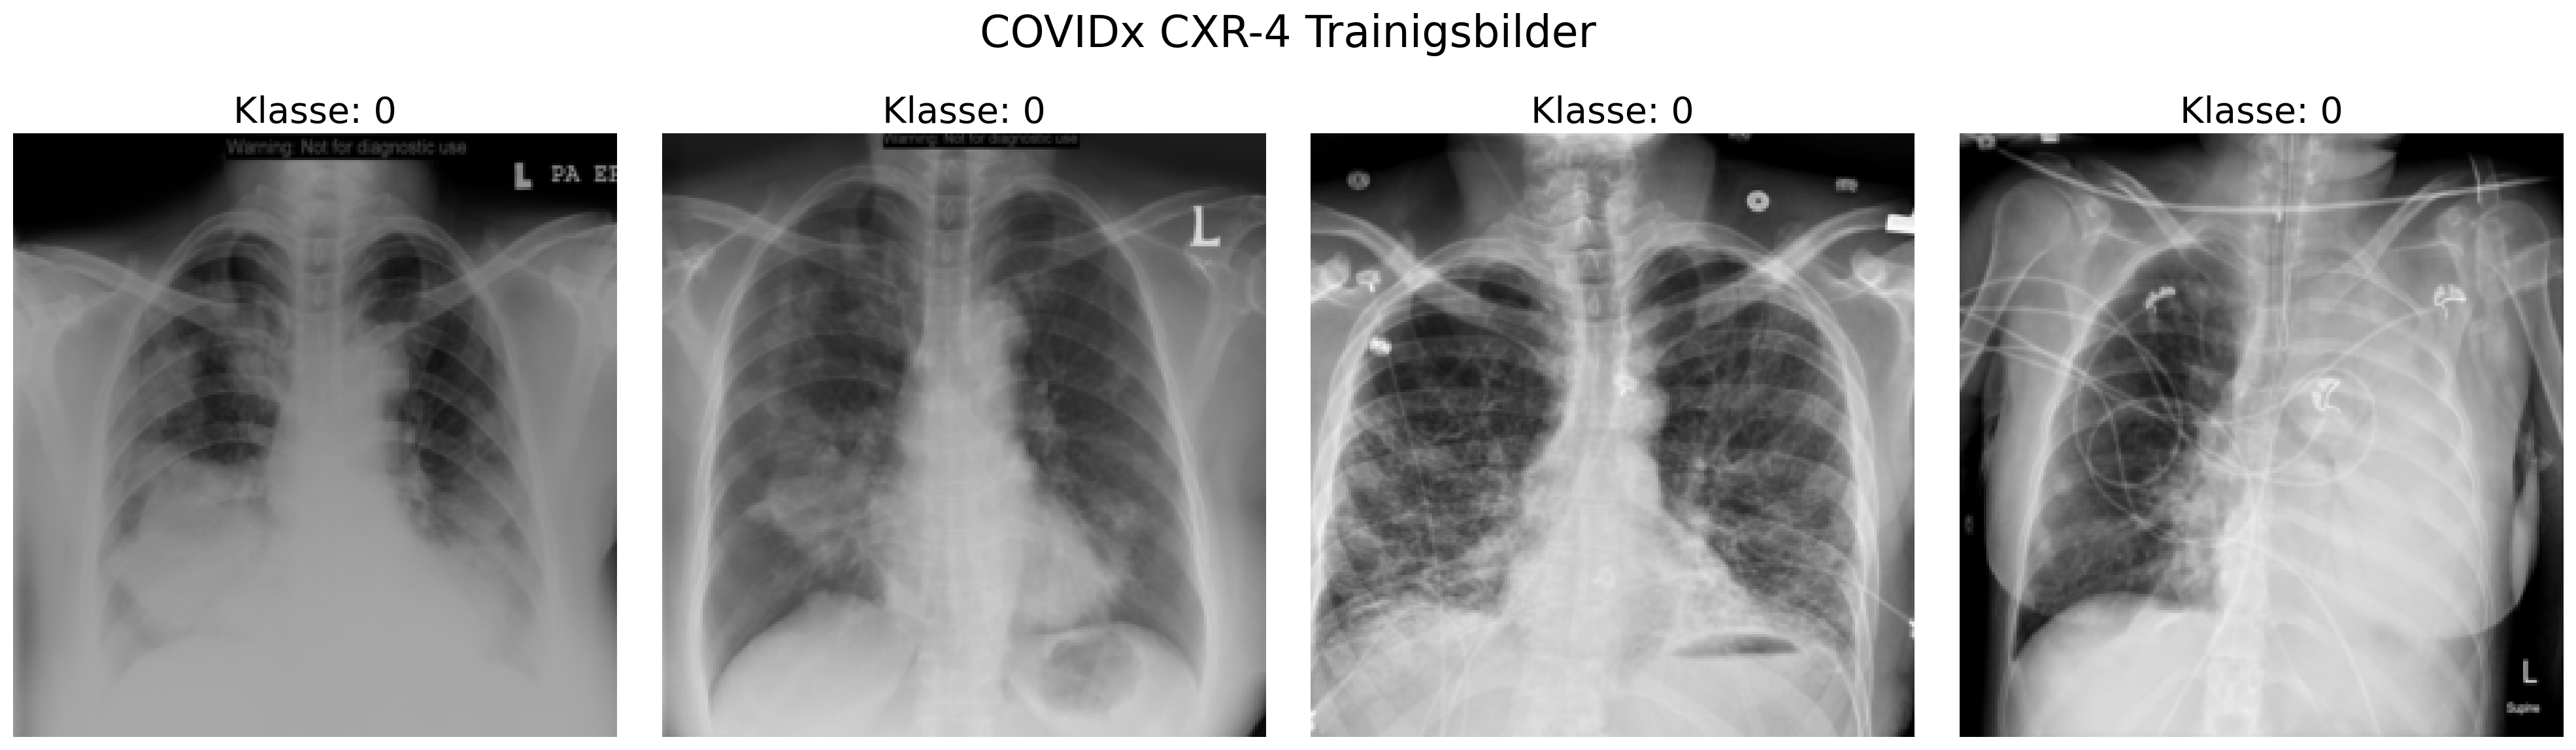
\includegraphics[width=\linewidth, height=4cm]{01-images/03-data/covid19-klasse0.png}
    \caption{Beispiele von negativen Covid Patienten vom COVIDx CXR-4 Datensatz}
    \label{fig:covid19-klasse0}
\end{figure}

\begin{figure}[H]
    \centering
    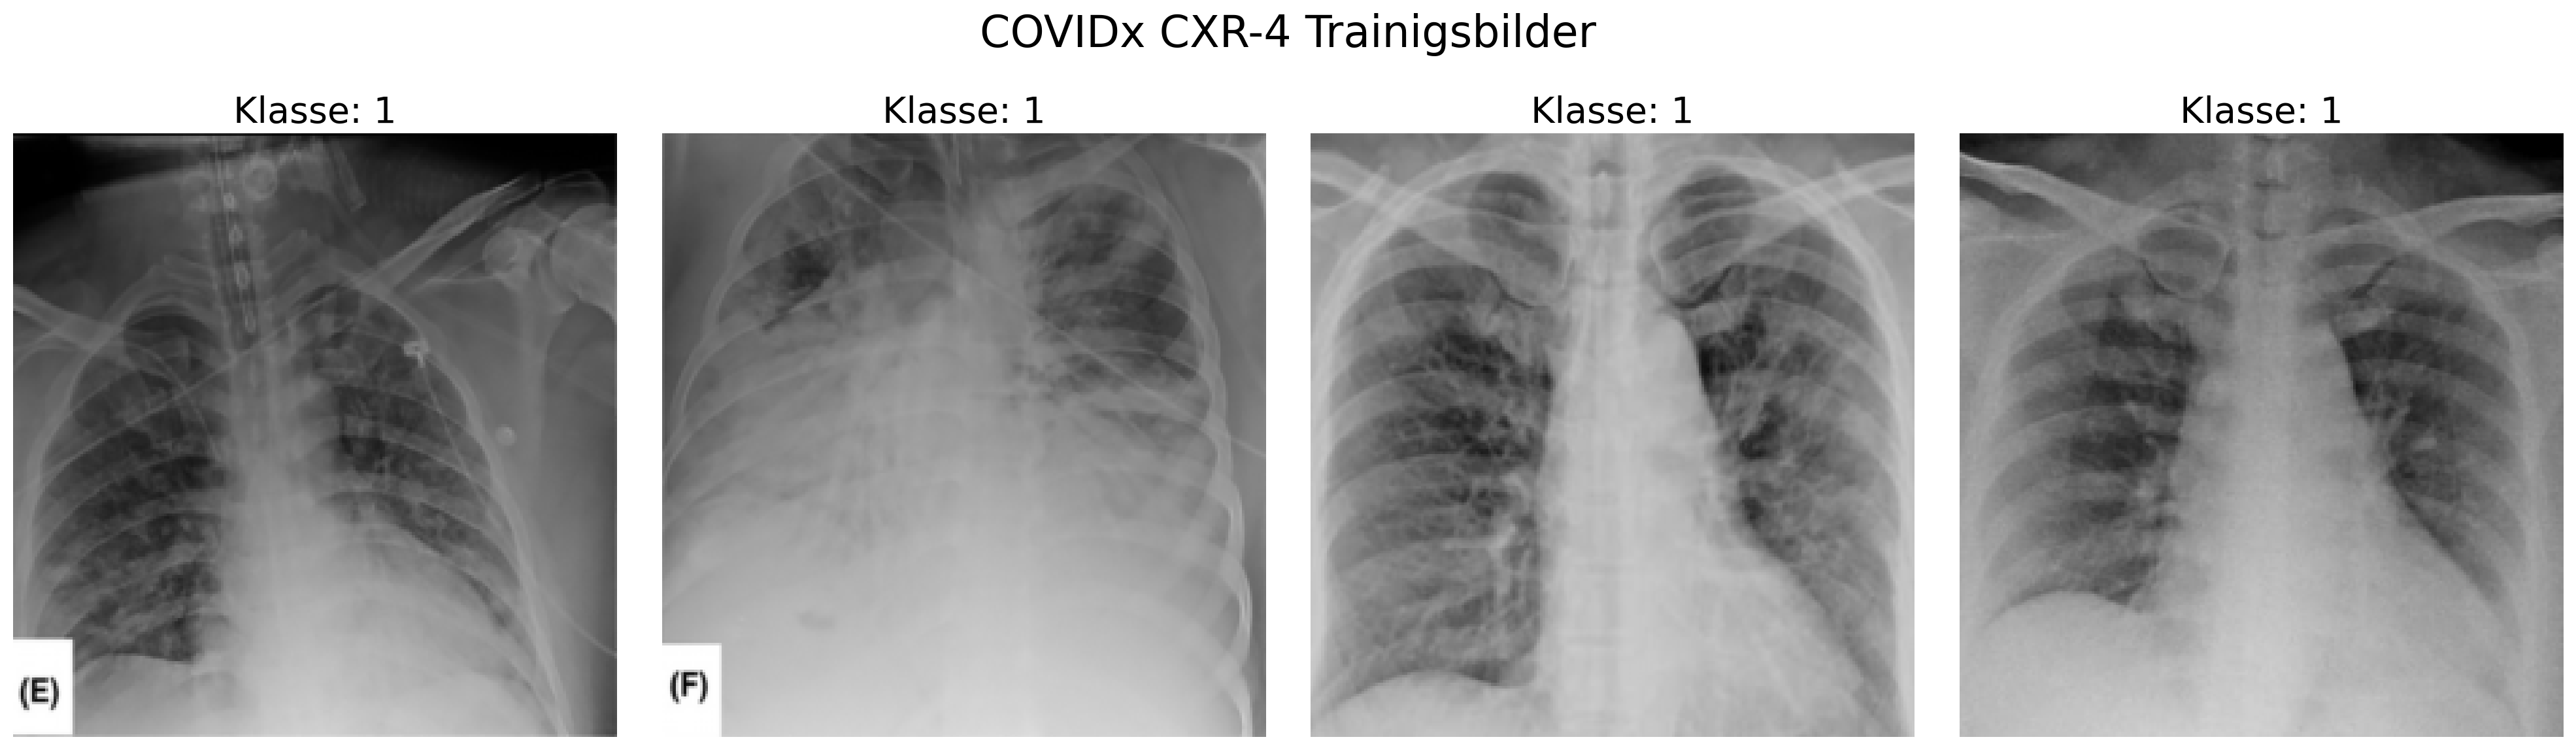
\includegraphics[width=\linewidth, height=4cm]{01-images/03-data/covid19-klasse1.png}
    \caption{Beispiele von positiven Covid Patienten vom COVIDx CXR-4 Datensatz}
    \label{fig:covid19-klasse1}
\end{figure}


\subsubsection{Datenpartitionierung} \label{chap:COVIDX-Partition}

Die Datenpartitionierung ist bereits durch die Struktur vorgegeben. Wir stellen fest, dass die Klassenverteilung von positiven und negativen Labels für die Validierung und den Testdatensets fast gleich verteilt ist, mit einem Verhältnis von 50\% positive sowie 50\% negative Fälle. 

\begin{table}[h]
\centering
\begin{tabular}{@{}cccccc@{}}
\toprule
Partition & \multicolumn{2}{c}{Anzahl Bilder} & \multicolumn{2}{c}{Klassenverteilung} & Positiv-Verhältnis\\ 
\cmidrule(lr){2-3} \cmidrule(lr){4-5} 
          & Absolut & Relativ & Positiv & Negativ & \\ 
\midrule
Train      & 67863 & 0.8001 & 57199 & 10664 & 0.8429 \\
Validation & 8473  & 0.0999 & 4241  & 4232  & 0.5005 \\
Test       & 8482  & 0.1000 & 4241  & 4241  & 0.5000 \\ 
\bottomrule
\end{tabular}
\caption{Klassenverteilung von COVIDX-CXR4}
\label{tab:covidx-klassenverteilung}
\end{table}

\subsubsection{Datenexploration}


In den dargestellten Histogrammen sehen wir die Pixelverteilung der Röntgenbilder von positiven \ref{fig:covid19-klasse1} und negativen \ref{fig:covid19-klasse0} Patienten. Jedes Histogramm repräsentiert die Intensitätsverteilung der Pixelwerte in den jeweiligen Röntgenaufnahmen. Die x-Achse jedes Histogramms zeigt die Grauwertintensität von 0 bis 255, während die y-Achse die Anzahl der Pixel für jede Intensität darstellt. 

\begin{figure}[ht]
    \centering
    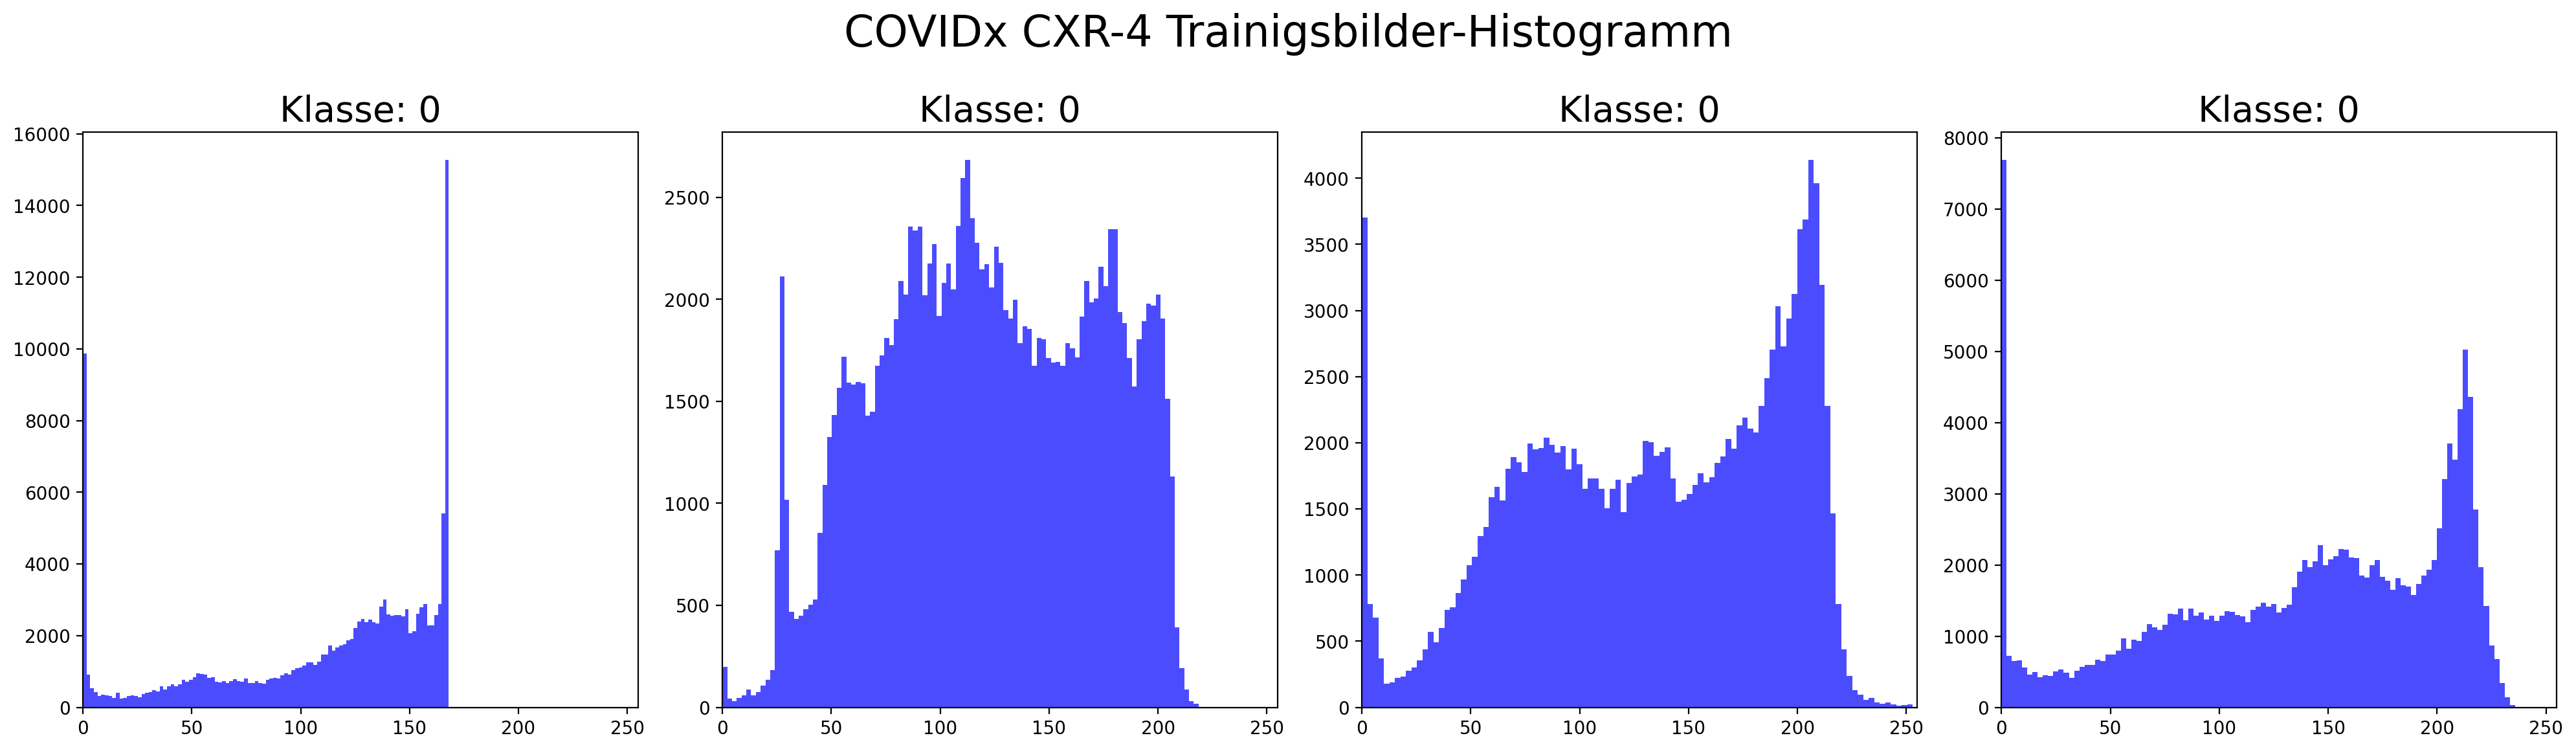
\includegraphics[width=\linewidth, height=4cm]{01-images/03-data/covid19-klasse0-hist.png}
    \caption{Histogramm der Pixelverteilung von Abbildung \ref{fig:covid19-klasse0}}
    \label{fig:covid19-klasse0-hist}
\end{figure}

\begin{figure}[ht]
    \centering
    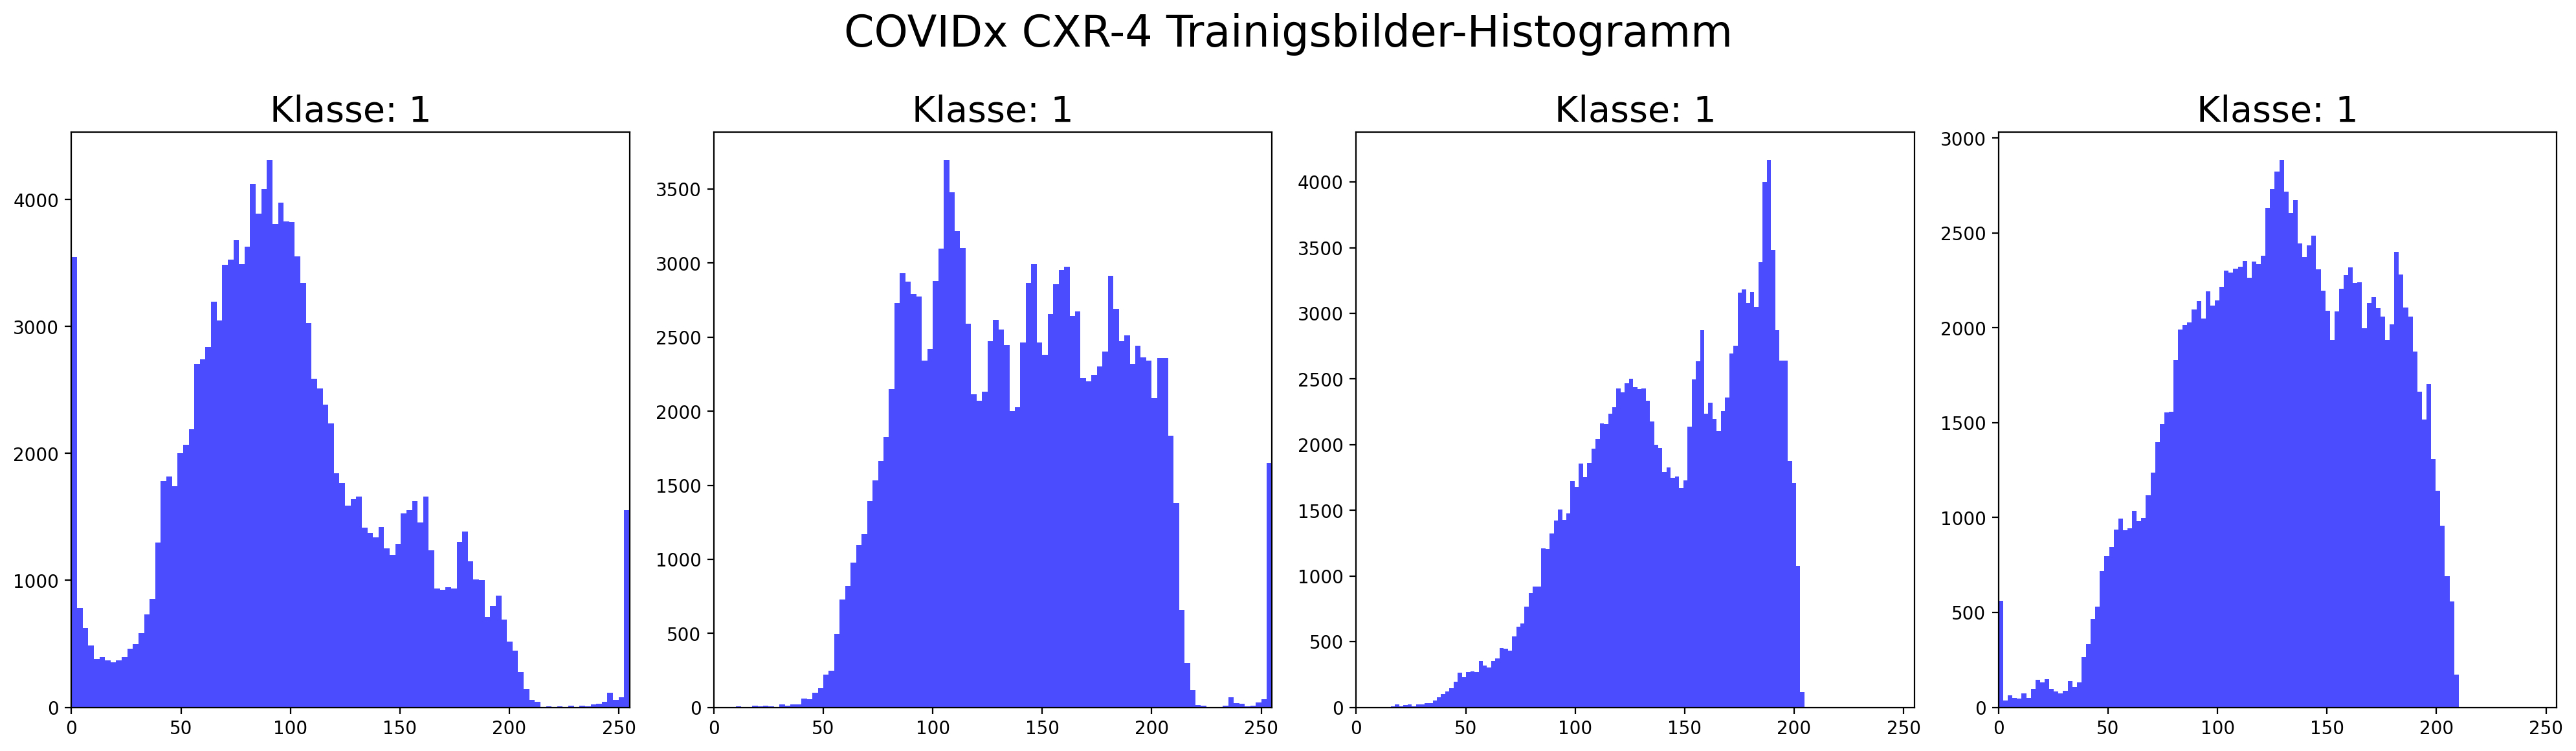
\includegraphics[width=\linewidth, height=4cm]{01-images/03-data/covid19-klasse1-hist.png}
    \caption{Histogramm der Pixelverteilung von Abbildung \ref{fig:covid19-klasse1}}
    \label{fig:covid19-klasse1-hist}
\end{figure}

Die Histogramme der Röntgenbilder variieren stark von Bild zu Bild. Tiefe Pixelwerte repräsentieren vermutlich Weichgewebe, während höhere Pixelwerte harte Knochengewebe darstellen

\subsection{Datenverteilung \& Testperofmance} \label{chap:Datenverteilung-Testperformance-covidx}

Im Verlauf unserer Arbeit stellten wir fest, dass die Performance-Metriken der Testdaten von Covidx nicht den erwarteten Werten entsprechen. Daher führten wir eine umfassende explorative Analyse der Trainings-, Validierungs- und Testdaten durch, um potenzielle Ursachen für diese Diskrepanzen zu identifizieren. In den folgenden Kapiteln \ref{chap:Pixelverteilung-TestProblemEda1-covidx}, \ref{chap:Differenzenbilder-TestProblemEda2-covidx} und \ref{chap:FeatureMaps-TestProblemEda3-covidx} zeigen wir die Resultate der Untersuchungen.

\todo{vorab weg die Resultate schon hier erwaehnen}

\subsubsection{Pixelverteilung} \label{chap:Pixelverteilung-TestProblemEda1-covidx}

Um die Verteilung der Pixelwerte zu analysieren, flachen wir die Bilder zu einem eindimensionalen Vektor ab. Diese Vektoren repräsentieren alle Bilder einer jeweiligen Datenpartition. Die resultierenden Daten visualisieren wir mithilfe von Histogrammen, wie in Abbildung \ref{fig:hist-datapartition-covid} dargestellt.

\begin{figure}[ht]
    \centering
    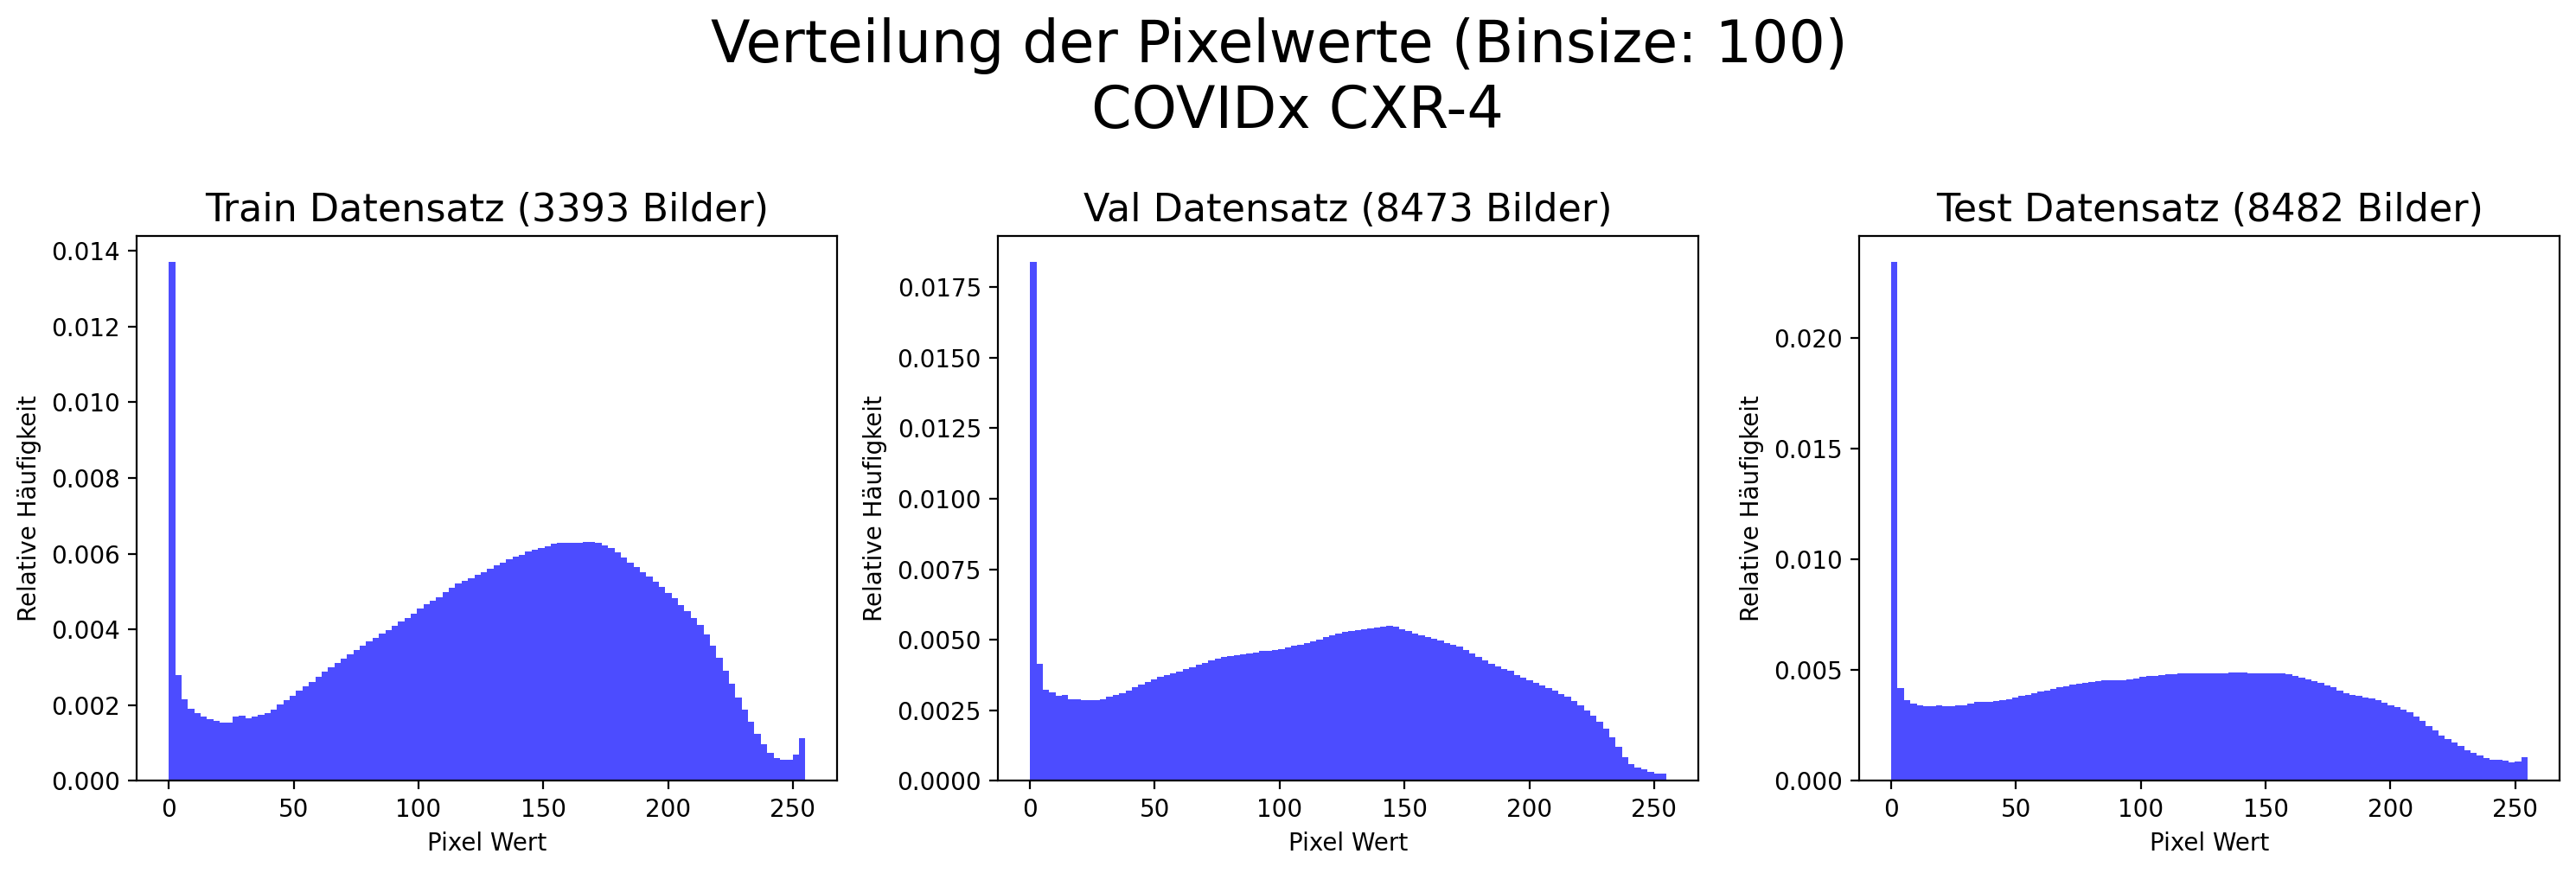
\includegraphics[width=\linewidth, height=5cm]{01-images/03-data/covid-Pixelverteilung-Partitionen.png}
    \caption{Histogramme der Pixelverteilung von Covid in jeder Datenpartition}
    \label{fig:hist-datapartition-covid}
\end{figure}

Die Histogramme verdeutlichen, dass Pixelwerte nahe null, welche schwarzen Pixeln entsprechen, häufig auftreten, was bei Röntgenaufnahmen üblich ist. Besonders auffällig ist der Gipfel, der seinen Höhepunkt bei einem Pixelwert von etwa 180 erreicht. Dieser Gipfel ist auch im Validierungsdatensatz vorhanden, allerdings weniger ausgeprägt und abgeflacht. Im Testdatensatz ist dieser Gipfel nahezu nicht vorhanden. Stattdessen ist am Ende der Verteilung ein leichter Anstieg zu beobachten, der auf die Präsenz von weissen Pixelwerten hinweist. Die Verteilung der Pixelwerte in den Trainings- und Validierungsdaten weisen ein ähnliches Muster auf, jedoch mit unterschiedlichen Intensitäten. Dies könnte auf eine Variation in der Bildaufnahme  zwischen den Partitionen deuten. Der deutliche Unterschied im Testdatensatz, insbesondere das fast völlige Fehlen des typischen Gipfels, könnte auf eine unterschiedliche Charakteristik der Bilder oder eine andere Verteilung in dieser Partition hindeuten. Es lässt sich nicht definitiv ausschliessen oder bestätigen, dass die Testpartitionen einer anderen Verteilung folgen. Dies könnte auf verschiedene Faktoren wie Belichtungszeiten, Sensoreinstellungen oder sogar auf die Art und Weise der Datensammlung, beispielsweise durch unterschiedliche Maschinen zurückzuführen sein.

\subsubsection{Differenzbilder} \label{chap:Differenzenbilder-TestProblemEda2-covidx}

Differenzbilder werden verwendet, um den durchschnittlichen Pixelwert innerhalb jeder Datenpartition in einer festgelegten Dimension von 224 x 224 Pixeln zu berechnen. Diese spezifische Dimension wurde aufgrund der Anforderungen des Preprocessing-Schrittes in unserer Analyse gewählt. Durch die Berechnung des Mittelwerts über alle Bilder einer Partition können diese Bilder dann als Heatmaps visualisiert werden. Ziel dieser Visualisierungsmethode ist es, die Unterschiede zwischen den Partitionen auf eine visuell zugängliche Weise darzustellen und dadurch potenzielle Auffälligkeiten oder Muster zu identifizieren.

\begin{figure}[ht]
    \centering
    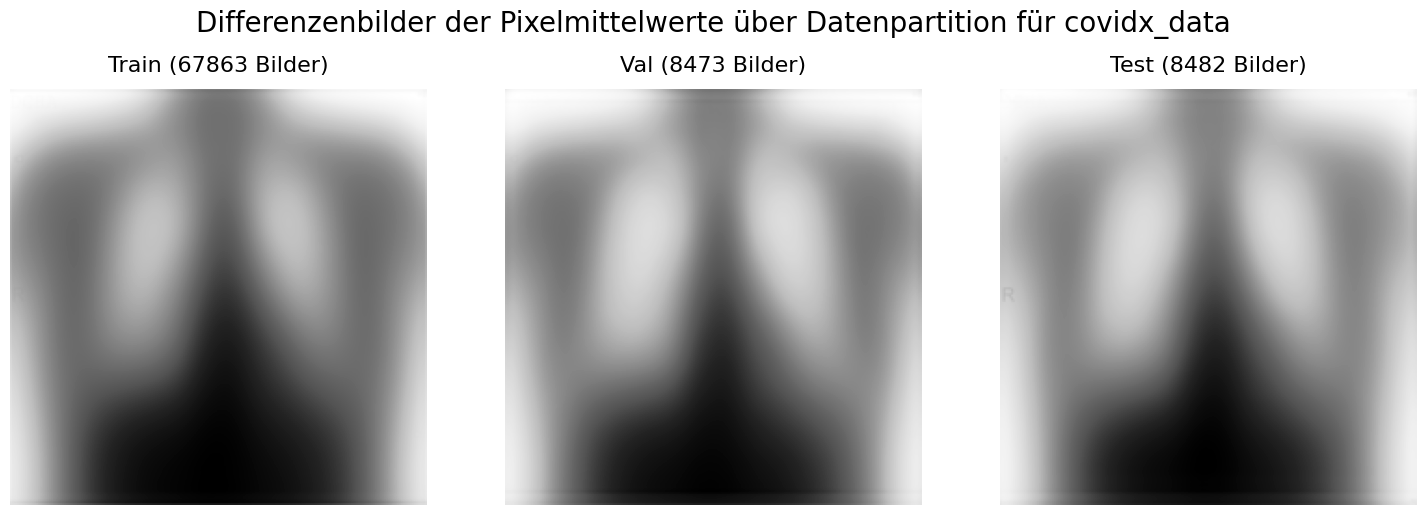
\includegraphics[width=\linewidth, height=5cm]{01-images/03-data/covid-Differenzenbilder-Partition.png}
    \caption{Differenzbilder von Covid in jeder Datenpartition}
    \label{fig:differenzenbilder-datapartition-covid}
\end{figure}

In der Analyse der Differenzbilder der Pixelmittelwerte über die verschiedenen Datenpartitionen für den Covid Datensatz zeigt sich, dass Unterschiede zwischen Trainings,- Validierung,- Testpartition vorhanden sind. Dies ist jedoch nicht verwunderlich, da die Bilder von unterschiedlichen Personen stammen und der Datensatz eine Sammlung von Covid Bilder ist. Die anatomischen Strukturen, wie die Rippenknochen, sind über alle Partitionen hinweg deutlich zu erkennen. 

\subsubsection{Feature Maps \& PCA} \label{chap:FeatureMaps-TestProblemEda3-covidx}

Im Rahmen unserer Analyse nutzen wir ein ResNet50-Modell, das zum einen durch PyTorch vorab trainiert und zum anderen speziell auf unseren Datensatz angepasst wurde. Besonderes Augenmerk liegt auf der Featureextraktion aus dem vorletzten Layer des Modells, direkt vor dem Klassifikationslayer. Die in diesem Schritt gewonnenen Vektoren, auch als Feature Maps bekannt, durchlaufen einer PCA Dimensionsreduktion. Ziel dieser Reduktion ist es, die Dimensionalität der Daten auf zwei Dimensionen zu reduzieren, um eine Visualisierung der verschiedenen Datenpartitionen zu ermöglichen. Die Interpretation erweist sich als sehr komplex und die Ergebenisse sind nur schwer zu interpretieren. 


\newpage